\section{előadás (2025. december 2.)}
\subsubsection*{Ütemezés}

Adott munkák $M = \{m_1, m_2, \cdots, m_n\}$ halmaza, és minden $m_i \in M$-hez:

\begin{itemize}
    \item $t_i$: ennyi ideig tart elvégezni
    \item $d_i$: határidő
    \item $w_i$: munkadíj
\end{itemize}

($\geq 0$ egészek)

Mely munkákat vállaljuk el a max. összdíjért?

\begin{itemize}[label=$\rightarrow$]
    \item egyszerre csak egy munkát lehet végezni
    \item nem lehet félbeszakítani
    \item határidőre be kell fejezni
\end{itemize}

Az $m_{i_1}, m_{i_2}, \cdots, m_{i_k}$ kiválasztott munkák egy megengedett ütemezése: megadunk $S_{i_1}, f_{i_1}$ értékeket, amire:
\begin{flalign*}
    &0 \leq S_{i_1}, f_{i_1} = S_{i_1} + t_{i_1}, f_{i_1} \leq d_{i_1} &&\\
    &f_{i_1} \leq S_{i_2}, f_{i_2} = S_{i_2} + t_{i_2}, f_{i_2} \leq d_{i_2} &&\\
    &f_{i_2} \leq S_{i_3}, f_{i_3} = S_{i_3} + t_{i_3}, f_{i_3} \leq d_{i_3} &&\\
    &\vdots &&\\
    &f_{i_{k-1}} \leq S_{i_{k}}, f_{i_{k}} = S_{i_{k}} + t_{i_{k}}, f_{i_{k}} \leq d_{i_{k}} &&
\end{flalign*}

Szeretnénk az $M$ olyan részhalmazát választani, aminek van megengedett ütemezése és $\overset{k}{\underset{l=1}{\sum}} w_{i_k}$ maximális.

Ez NP-nehéz feladat.
Létezik DP algoritmus a feladat megoldására.

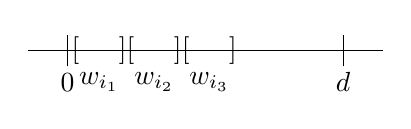
\begin{tikzpicture}
\draw (0, 0) -- (4.5, 0);
\draw (0.5, -0.2) -- (0.5, 0.2);
\draw (4, -0.2) -- (4, 0.2);

\node at (0.5, -0.4){$0$};
\node at (4, -0.4){$d$};

\node at (0.6, 0) {[};
\node at (1.2, 0) {]};
\node at (0.9, -0.4) {$w_{i_1}$};

\node at (1.3, 0) {[};
\node at (1.9, 0) {]};
\node at (1.6, -0.4) {$w_{i_2}$};

\node at (2.0, 0) {[};
\node at (2.6, 0) {]};
\node at (2.3, -0.4) {$w_{i_3}$};

\end{tikzpicture}

Speciális eset: $d_1 = d_2 = \cdots = d_n = d$.
Minden határidő ugyanaz $\rightarrow$ hátizsák probléma $t_i$ súlyokkal, $w_i$ értékkel, $d$ kapacitással.

Egy másik speciális eset: $w_1 = w_2 = \cdots = w_n$.
Cél: legtöbb munka elvégzése.
Erre van $\mathcal{O}(n \log n)$-es MOHÓ ALGORITMUS.

Mohó algoritmus az ütemezési probléma speciális esetére:\\
Feltehetjük, hogy $d_1 \leq d_2 \leq \cdots \leq d_n$.
Egy $H$ halmazba fogjuk gyűjteni a kiválasztott munkákat.
Kezdetben legyen $H = \oslash$.
Egymás után vesszük hozzá $H$-hoz az $m_1$ munkákat. $i = 1,2,3, \cdots$.

Ha az $m_i$ munka bevételével $\underset{m_j \in H}{\sum} t_j > d_i$ adódik, akkor töröljük $H$-ból a leghosszabb elvégzési idejűt.

Végül a $H$-beli feladatokat ütemezzük a 0. időpillanattól szünet nélkül a határidők szerint növekvő sorrendben (kanonikus ütemezés).

\begin{tikzpicture}
\draw (0, 0) -- (5.5, 0);

\draw (0.5, -0.2) -- (0.5, 0.2);
\draw (1.2, -0.2) -- (1.2, 0.2);
\draw (1.9, -0.2) -- (1.9, 0.2);
\draw (2.6, -0.2) -- (2.6, 0.2);

\draw (3.8, -0.2) -- (3.8, 0.2);
\draw (4.5, -0.2) -- (4.5, 0.2);

\node at (0.5, -0.4){$0$};
\node at (0.9, 0.4){$t_1$};
\node at (1.6, 0.4){$t_2$};
\node at (2.3, 0.4){$t_3$};
\node at (3.0, -0.4){$\cdots$};
\node at (3.4, 0.4){$t_{i-1}$};
\node at (4.2, 0.4){$t_i$};

\draw[-Latex] (4.2, -0.8) -- (4.2, -0.1);
\node at (4.2, -1) {$d_{i-1} \leq d_i$};
\end{tikzpicture}

\textbf{Állítás:} $H$-ban minden munka befejeződik legkésőbb a határidőre.\\
\textbf{Bizonyítás:} triviális.

\clearpage
\textbf{Állítás:} $H$ optimális ütemezés az adott munkákra nézve.\\
\textbf{Bizonyítás:}\\
Indukció $n$-re ($|M| = n$)

$n = 1$: triviális

Most tegyük fel, hogy $n > 1$ és a mohó algoritmus optimális ütemezést ad $\leq n-1$ munka esetén.

Ha $H$ tartalmazza az összes munkát, akkor optimális $\rightarrow$ kész vagyunk.

Tegyük fel, hogy $H$ nem az összes munkát tartalmazza, és legyen $m_k$ az a munka, amit először törölt a mohó algoritmus, mondjuk az $m_i$ munka hozzávételekor.

\textbf{Állítás:} van olyan $\mathcal{O}$ optimális kanonikus ütemezés, hogy $m_k$ ebben sem szerepel.\\
\textbf{Bizonyítás:} hamarosan

Hogyan használhatjuk ezt $H$ optimalitásának bizonyítására?

Nyilván: $|H| \leq |\mathcal{O}|$* mert $\mathcal{O}$ optimális.

Tekintsük most azt a feladatot, hogy $m_1, m_2, \cdots, m_{k-1}, m_{k+1}, \cdots, m_n = M'$ (eggyel kevesebb munkánk van) munkákat kell ütemezni.

Ekkor a mohó algoritmus itt is pont a $H$ ütemezést fogja adni.

Az indukciós feltevés miatt itt ($M'$ munkák esetén) a mohó algoritmus optimális ütemezést ad.

$\mathcal{O}$ az $M'$ munkákra megengedett ütemezés (mert nincs benne $m_k$).
Emiatt $\mathcal{O} \leq |H|$ és * (azaz $|H| \leq |\mathcal{O}|$) miatt $|H| = |\mathcal{O}|$, tehát $H$ is optimális ütemezés az $M$ munkákra.

\textbf{Költségek:}
\begin{enumerate}
    \item kezdeti rendezés: $\mathcal{O}(n \log n)$
    \item $H$ manipulációja:
    \begin{itemize}
        \item tároljuk $H$ elemeit egy (max) kupacban
        \item egy segédváltozóban tároljuk a $H$-beli munkák össz-elvégzési idejét
    \end{itemize}
\end{enumerate}

Műveletek $H$-val:
\begin{itemize}
    \item $m_i$ bevétele $H$-ba
    \begin{itemize}[label=$\rightarrow$]
        \item bevesszük a kupacban $\leftarrow \mathcal{O}(\log n)$
        \item segédváltozó $t_i$-vel növelve $\leftarrow \mathcal{O}(1)$
        \item vizsgálat: segédváltozó $\overset{?}{>} d_i$ $\leftarrow \mathcal{O}(1)$
    \end{itemize}
    \item $m_k$ törlése $H$-ból
    \begin{itemize}[label=$\rightarrow$]
        \item remMax $\leftarrow \mathcal{O}(\log n)$
        \item segédváltozó csökken $t_k$-val $\leftarrow \mathcal{O}(1)$
    \end{itemize}
\end{itemize}

$\Rightarrow$ $n$ darab munkára $\mathcal{O}(n \log n)$ költség

\textbf{Állítás:} van olyan $\mathcal{O}$ optimális kanonikus ütemezés, hogy $m_k$ ebben sem szerepel.\\
\textbf{Bizonyítás:} tfh. $\mathcal{O}$ optimális kanonikus ütemezés és $m_k$ benne van $m_k$ választásából adódik, hogy az $m_i$ bevételekor távolítottuk el $m_k$-t $H$-ból.

$\overset{i}{\underset{j=1}{\sum}} t_i > d_i$

Emiatt az $m_1, m_2, \cdots, m_{i}$ munkák valamelyike hiányzik $\mathcal{O}$-ból.

Legyen $m_l$ az a munka, ami nincs $\mathcal{O}$-ban ($1 \leq l \leq i, l \neq k$).

Cseréljük ki $\mathcal{O}$-ban az $m_k$ munkát $m_l$-re, ütemezzük kanonikusan, legyen ez $\mathcal{O}^*$.

\clearpage
\textbf{Állítás:} $\mathcal{O}^*$-ban is minden munka befejeződik határidőre.\\
\textbf{Bizonyítás:} $m_k$ választása miatt $t_k \geq t_l$.

$\mathcal{O}$:
\raisebox{-.5\height}{
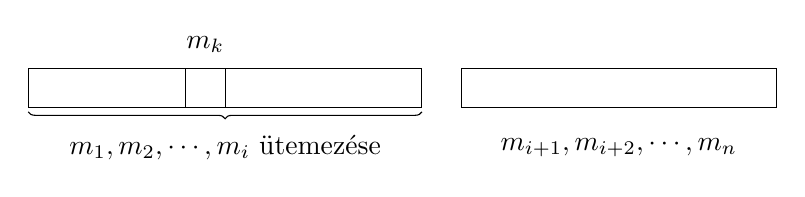
\begin{tikzpicture}
\draw (0,0) rectangle ++(5,0.5);
\draw (5.5,0) rectangle ++(4,0.5);

\draw[decoration={brace, raise=0.05cm, mirror}, decorate] (0, 0) -- (5, 0);
\node at (2.5, -0.5) {$m_1, m_2, \cdots, m_i$ ütemezése};
\node at (7.5, -0.5) {$m_{i+1}, m_{i+2}, \cdots, m_n$};

\draw (2.0, 0) -- (2.0, 0.5);
\draw (2.5, 0) -- (2.5, 0.5);
\node at (2.25, 0.8) {$m_k$};
\end{tikzpicture}
}

$\mathcal{O}^*$:
\raisebox{-.85\height}{
\begin{tikzpicture}
\draw (0,0) rectangle ++(5,0.5);
\draw (5.5,0) rectangle ++(4,0.5);
\node at (2.5, -0.3) {$m_k$-t lecseréltük a nála};
\node at (2.5, -0.7) {rövidebb idejű $m_l$-re};
\node at (3.0, -1.7) {minden munka vagy helyben maradt,};
\node at (3.0, -2.1) {vagy balra csúszott $\rightarrow$ kész lesz mind};

\draw[-Latex] (2.5, -1.0) -- (2.5, -1.5);

\end{tikzpicture}
}

$\mathcal{O}^*$ is optimális, és $\mathcal{O}^*$ nem tartalmazza az $m_k$ munkát. QED

